% ---------------------------------------------------------------------------
% Worked example: one document end to end.
% % ---------------------------------------------------------------------------
% Worked example: one document end to end.
% % ---------------------------------------------------------------------------
% Worked example: one document end to end.
% % ---------------------------------------------------------------------------
% Worked example: one document end to end.
% \input{figures/fig_sandy_worked_example} — expects graphicx; one-column float.
% Asset: fig_sandy_worked_example.pdf, regenerated by
% figures/make_fig_sandy_worked_example.py from fig_sandy_source_text.txt,
% fig_sandy_extraction.json and fig_sandy_footprint.pdf.
% Rendered size is 3.15 x 6.60 in; scale with width=\columnwidth.
% ---------------------------------------------------------------------------
\begin{figure}[t]
  \centering
  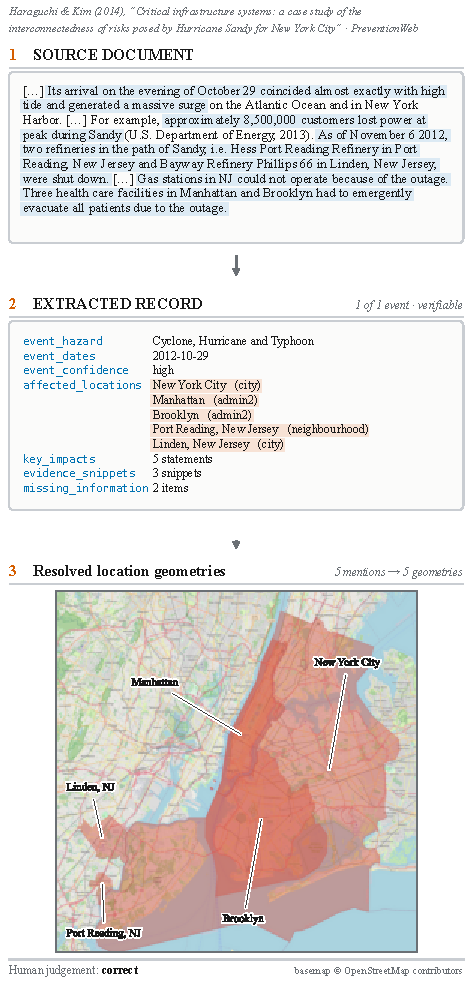
\includegraphics[width=\columnwidth]{figures/fig_sandy_worked_example}
  \caption{One document end to end. (1) An excerpt of the 12{,}000-character
  window passed to the model; shading marks the spans it returned in
  \texttt{evidence\_snippets}. (2) The resulting record, abridged:
  \texttt{key\_impacts}, \texttt{evidence\_snippets} and
  \texttt{missing\_information} are shown as counts. (3) The five location
  strings after geocoding, as the union of their resolved geometries --- the
  city, borough and neighbourhood levels overlap, and the two New Jersey
  refinery sites resolve to separate polygons. Every element is recoverable
  from the emitted row: the snippet, the location string and admin level it
  came from, and the geometry it resolved to. This record was judged correct
  (\S\ref{sec:validation}). Basemap \copyright{} OpenStreetMap contributors.}
  \label{fig:worked-example}
\end{figure}
 — expects graphicx; one-column float.
% Asset: fig_sandy_worked_example.pdf, regenerated by
% figures/make_fig_sandy_worked_example.py from fig_sandy_source_text.txt,
% fig_sandy_extraction.json and fig_sandy_footprint.pdf.
% Rendered size is 3.15 x 6.60 in; scale with width=\columnwidth.
% ---------------------------------------------------------------------------
\begin{figure}[t]
  \centering
  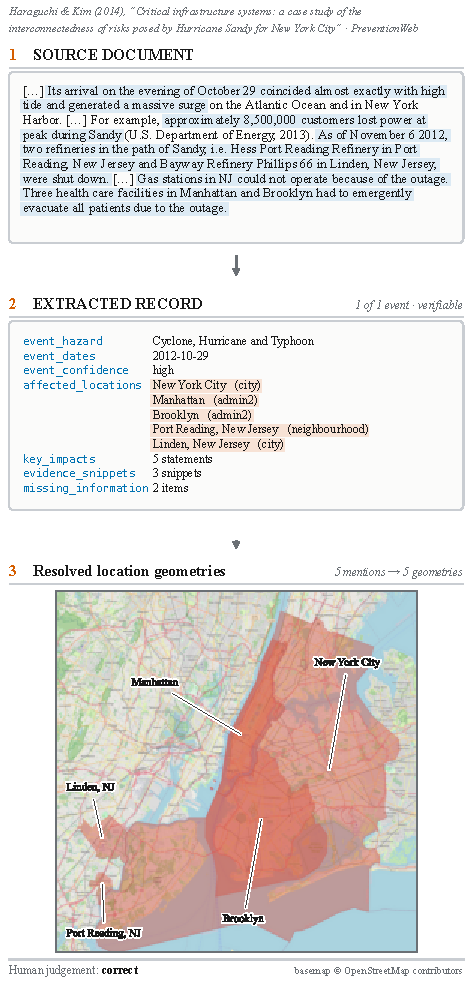
\includegraphics[width=\columnwidth]{figures/fig_sandy_worked_example}
  \caption{One document end to end. (1) An excerpt of the 12{,}000-character
  window passed to the model; shading marks the spans it returned in
  \texttt{evidence\_snippets}. (2) The resulting record, abridged:
  \texttt{key\_impacts}, \texttt{evidence\_snippets} and
  \texttt{missing\_information} are shown as counts. (3) The five location
  strings after geocoding, as the union of their resolved geometries --- the
  city, borough and neighbourhood levels overlap, and the two New Jersey
  refinery sites resolve to separate polygons. Every element is recoverable
  from the emitted row: the snippet, the location string and admin level it
  came from, and the geometry it resolved to. This record was judged correct
  (\S\ref{sec:validation}). Basemap \copyright{} OpenStreetMap contributors.}
  \label{fig:worked-example}
\end{figure}
 — expects graphicx; one-column float.
% Asset: fig_sandy_worked_example.pdf, regenerated by
% figures/make_fig_sandy_worked_example.py from fig_sandy_source_text.txt,
% fig_sandy_extraction.json and fig_sandy_footprint.pdf.
% Rendered size is 3.15 x 6.60 in; scale with width=\columnwidth.
% ---------------------------------------------------------------------------
\begin{figure}[t]
  \centering
  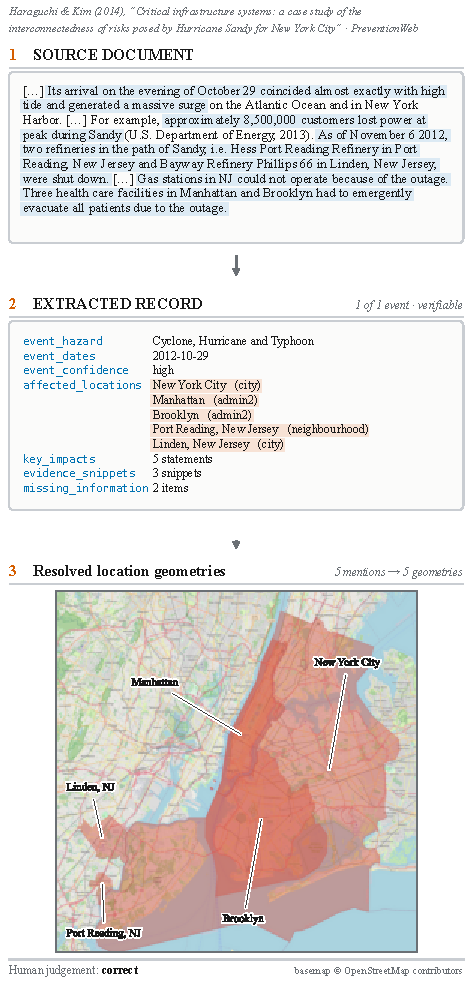
\includegraphics[width=\columnwidth]{figures/fig_sandy_worked_example}
  \caption{One document end to end. (1) An excerpt of the 12{,}000-character
  window passed to the model; shading marks the spans it returned in
  \texttt{evidence\_snippets}. (2) The resulting record, abridged:
  \texttt{key\_impacts}, \texttt{evidence\_snippets} and
  \texttt{missing\_information} are shown as counts. (3) The five location
  strings after geocoding, as the union of their resolved geometries --- the
  city, borough and neighbourhood levels overlap, and the two New Jersey
  refinery sites resolve to separate polygons. Every element is recoverable
  from the emitted row: the snippet, the location string and admin level it
  came from, and the geometry it resolved to. This record was judged correct
  (\S\ref{sec:validation}). Basemap \copyright{} OpenStreetMap contributors.}
  \label{fig:worked-example}
\end{figure}
 — expects graphicx; one-column float.
% Asset: fig_sandy_worked_example.pdf, regenerated by
% figures/make_fig_sandy_worked_example.py from fig_sandy_source_text.txt,
% fig_sandy_extraction.json and fig_sandy_footprint.pdf.
% Rendered size is 3.15 x 6.60 in; scale with width=\columnwidth.
% ---------------------------------------------------------------------------
\begin{figure}[t]
  \centering
  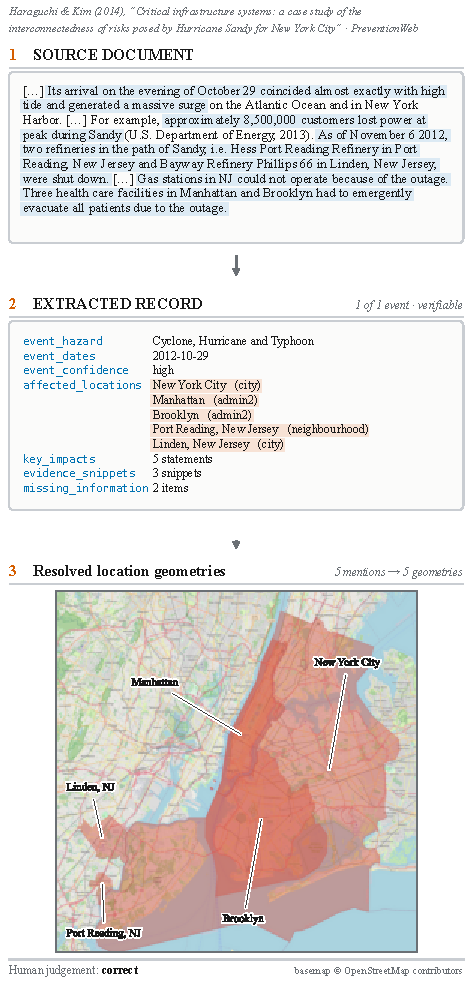
\includegraphics[width=\columnwidth]{figures/fig_sandy_worked_example}
  \caption{One document end to end. (1) An excerpt of the 12{,}000-character
  window passed to the model; shading marks the spans it returned in
  \texttt{evidence\_snippets}. (2) The resulting record, abridged:
  \texttt{key\_impacts}, \texttt{evidence\_snippets} and
  \texttt{missing\_information} are shown as counts. (3) The five location
  strings after geocoding, as the union of their resolved geometries --- the
  city, borough and neighbourhood levels overlap, and the two New Jersey
  refinery sites resolve to separate polygons. Every element is recoverable
  from the emitted row: the snippet, the location string and admin level it
  came from, and the geometry it resolved to. This record was judged correct
  (\S\ref{sec:validation}). Basemap \copyright{} OpenStreetMap contributors.}
  \label{fig:worked-example}
\end{figure}
